 % Theory of elasticity and failure
 \chapter{Elasticity and failure}
 To have a framework upon which to discuss failure and fracture in methane hydrates, we need some theory of elasticity and failure of elastic materials. This will also be needed in order to be explicit about how stresses and strains are imposed on model systems.

 \section{Linear elasticity}
Since I will deal with possibly anisotropic matrials, I start with the general tensor form of Hooke's law, and then provide the simplifications resulting from an isotropic material.
The generalized Hooke's law	is:
\begin{equation}
	\sigma_{ij} = c_{ijkl}\epsilon_{kl}
\end{equation}
This law relates the Cauchy stress tensor $\sigma_{ij}$ to the strain tensor $\epsilon_{kl}$ in a linearly elastic material. All material properties are contained in the stiffnes tensor $c_{ijkl}$.
In this form, Hooke's law basically states that ``each component of the cauchy stress tensor depends linearly on all components of the strain tensor''. 

Hooke's law contains two tensors of rank 2 with 9 components each, and one tensor of rank 4 with 81 componens. Luckily, there are symmetries to be exploited. First, the Cauchy stress tensor is symmetric, which leads to $c_{ijkl} = c_{jikl}$. Second, the strain tensor is symmetric, so $c_{ijkl} = c_{ijlk}$. This means we are left with 6 independent combination of each of $ij$ and $kl$, and a total of 36 components. 

Using the rank reduction method of Voigt, the stess and strain matrices can be written as vectors:
\begin{equation}
	\uuline{\sigma} = 
	\begin{pmatrix}
	\sigma_{11} & \sigma_{12} & \sigma_{13} \\
	\sigma_{21} & \sigma_{22} & \sigma_{23} \\
	\sigma_{31} & \sigma_{32} & \sigma_{33} \\ 
	\end{pmatrix}
	\to 
	\vec{\sigma} = 
	\begin{pmatrix}
	\sigma_{11} \\ \sigma_{22} \\ \sigma_{33} \\ \sigma_{23} \\ \sigma_{13} \\ \sigma_{12}
	\end{pmatrix}
	\equiv
	\begin{pmatrix}
	\sigma_{1} \\ \sigma_{2} \\ \sigma_{3} \\ \sigma_{4} \\ \sigma_{5} \\ \sigma_{6}
	\end{pmatrix}
\end{equation}

\begin{equation}
	\uuline{\epsilon} = 
	\begin{pmatrix}
	\epsilon_{11} & \epsilon_{12} & \epsilon_{13} \\
	\epsilon_{21} & \epsilon_{22} & \epsilon_{23} \\
	\epsilon_{31} & \epsilon_{32} & \epsilon_{33} \\ 
	\end{pmatrix}
	\to 
	\vec{\epsilon} = 
	\begin{pmatrix}
	\epsilon_{11} \\ \epsilon_{22} \\ \epsilon_{33} \\ 2\epsilon_{23} \\ 2\epsilon_{13} \\ 2\epsilon_{12}
	\end{pmatrix}
	\equiv
	\begin{pmatrix}
	\epsilon_{1} \\ \epsilon_{2} \\ \epsilon_{3} \\ \epsilon_{4} \\ \epsilon_{5} \\ \epsilon_{6}
	\end{pmatrix}
\end{equation}

For the same reasons, the stiffness tensor can be recuced to rank 2 (I choose not to write out the complete stiffness tensor, only the reduced one):
\begin{equation}
	\vec{C} =
	\begin{pmatrix}
	C_{11} & C_{12} & C_{13} & C_{14} & C_{15} & C_{16} \\
	C_{21} & C_{22} & C_{23} & C_{24} & C_{25} & C_{26} \\
	C_{31} & C_{31} & C_{33} & C_{34} & C_{35} & C_{36} \\
	C_{41} & C_{42} & C_{43} & C_{44} & C_{45} & C_{46} \\
	C_{51} & C_{52} & C_{53} & C_{54} & C_{55} & C_{56} \\
	C_{61} & C_{62} & C_{63} & C_{64} & C_{65} & C_{66}
	\end{pmatrix}
\end{equation}
Hooke's law can now be written as a matrix equation:
\begin{equation}
	\vec{\sigma} = \vec{C}\vec{\epsilon}
\end{equation}

It actually turns out that the stiffness matrix is symmetric, because stress and strain are work-conjugates:
\begin{equation}
	\sigma_i = \frac{\partial u}{\partial \epsilon_i}
\end{equation}
Where $u$ is the energy density associated with the stress-strain configuration.
Insering this into Hooke's law gives:
\begin{equation}
	C_{ij}=\frac{\partial^2 u}{\partial \epsilon_i \partial \epsilon_j} = \frac{1}{V} \frac{\partial^2 U}{\partial \epsilon_i \partial \epsilon_j} 
\end{equation}
This latter relation is useful for estimating the stiffness matrix from molecular simulation, as strains are easy to impose, and energy is trivial to measure.

\subsection{Isotropic materials}
Isotropic materials can be described by two parameters: Youngs modulus $E$ and poissons ratio $\nu$. The nature of the definition of these quantities leads to the stiffness matrix for isotropic materials:
\begin{equation}
	\vec{C} = 
   	\frac{E}{(1+\nu)(1-2\nu)}
   	\begin{pmatrix}
		1-\nu & \nu & \nu & 0 & 0 & 0 \\
		\nu & 1-\nu & \nu & 0 & 0 & 0 \\
		   \nu & \nu & 1-\nu & 0 & 0 & 0 \\
		   0 & 0 & 0 & (1-2\nu)/2 & 0 & 0 \\
		   0 & 0 & 0 & 0 & (1-2\nu)/2 & 0 \\
		   0 & 0 & 0 & 0 & 0 & (1-2\nu)/2
	\end{pmatrix}
\end{equation}

\subsection{Plane strain and plane stress}
Plane strain and plane stress are conditions where a three-dimensional elastic problem can be analyzed as two-dimensional ones. The formal definitions of plane strain and plane stress are given in equations \ref{eq:plane_strain} and \ref{eq:plane_stress}, respectively.

\begin{equation}
\uuline \epsilon = 
\begin{pmatrix}
	\epsilon_{11} & \epsilon_{12} & 0 \\
	\epsilon_{21} & \epsilon_{22} & 0 \\
	0 & 0 & 0
\end{pmatrix}
\label{eq:plane_strain}
\end{equation}

\begin{equation}
\uuline \sigma = 
\begin{pmatrix}
	\sigma_{11} & \sigma_{12} & 0 \\
	\sigma_{21} & \sigma_{22} & 0 \\
	0 & 0 & 0
\end{pmatrix}
\label{eq:plane_stress}
\end{equation}

For plane strain, we allow a nonzero stress component $\sigma_{33}$, and likewise, for plane stress we allow a nonzero strain component $\epsilon_{33}$. However, these components can only be results of the analysis, they shall not enter the analysis. 


\section{Simple fracture mechanics}
In linear elastic fracture mechanics (LEFM), there are essentially two quantities that govern failure: The stress intensity factor $K$, and the energy release rate $G$. For the case of linear elastic materials, these are uniquely related.

\subsection{Modes of loading}
There are 3 loading modes: I =`opening', II = `sliding', III = `tearing'. 

\begin{figure}
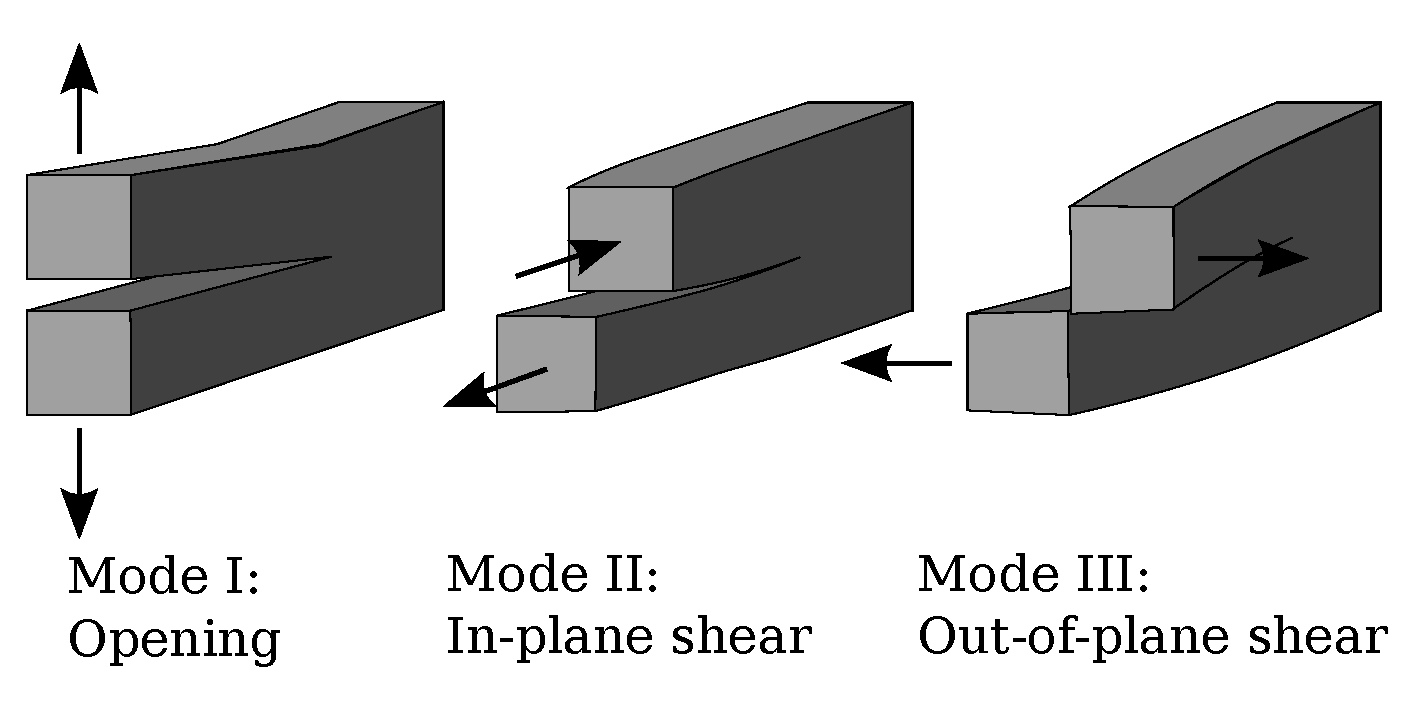
\includegraphics[width=\textwidth]{../figures/thesis/Fracture_modes_v2.pdf}
\caption{Three modes of crack separation. (``Fracture modes v2'' by Twisp - This vector image was created with Inkscape. Licensed under Public Domain via Wikimedia Commons)}
\end{figure}

\subsection{Stress intensity factors in anisotropic materials}
Simple fracture theory assumes that one only need one parameter to describe the fracture properties of a material, the critical stress intensity factor under tensile loading -- the fracture toughness. I will need a procedure to obtain that from molecular dynamics simulations. Having obtained the fracture area and the energy release rate, I can use the generalized irwin formula @citation to calculate the stress intensity factor. 

\begin{equation}
	G = \pi \vec{K}^T [\vec{H}] \vec{K} 
\end{equation}

Where $\vec{H}$ is a matrix that depends on the elastic properties of the material. This expression is valid for a plane crack propagating in two opposite directions with symmetric load with respect to the two directions of crack propagation.
To find the stress intensity factor for mode I loading, I only need to ensure a pure mode I loading situation, and obtain the element $H_{11}$. This matix element was worked out by \cite{Laubie2014}, and is:

\begin{equation}
	H_{11} = \frac{1}{2\pi} \sqrt{\frac{C_{11}}{C_{11}C_{33}-C^2_{13}}\left( \frac{1}{C_{44}} + \frac{2}{C_{13} + \sqrt{C_{11} C_{33}}}\right)}
\end{equation}

The stress intensity factor for mode I loading is the standard for fracture toughness measures. @ElegantClosingSentence

For the special case of isotropic materials under mode I loading, we recover a more familiar expression, Irwins formula for plane strains:

\begin{equation}
	K_c = \sqrt{\frac{EG_c}{1-\nu^2}}
\end{equation}

\subsection{Irwins criterion/formula @InvolvingEandGamma }

\subsection{Brittle and ductile materials}
In materials science, it is common to distinguish between brittle and ductile materials. According to Wikipedia, a material i brittle if it ``breaks without significant strain'', whereas ductility is ``a solid material's ability to deform under tensile stress''. Deformation in this context is plastic. It is actually hard to come along a more satisfying definition -- ductility and brittleness seems to be the kind of knowledge that everyone in the field have, but no one writes down as an equation. Throughout this thesis, I will use the term brittle -- by which i will be meaning ideally brittle -- about failure where the material acts completely elastic when subected to strain, until it suddenly breaks over essentialy no change in the strain.

\begin{figure}
\centering
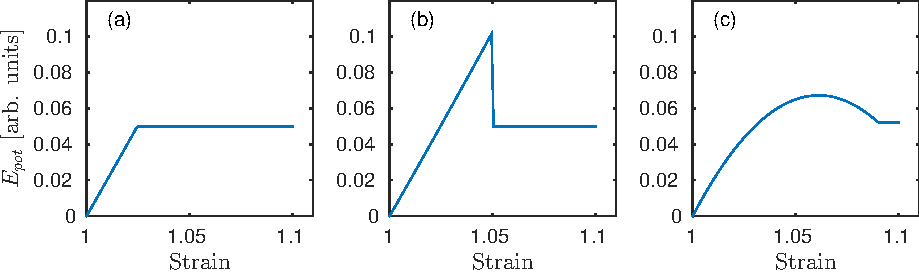
\includegraphics[width=\textwidth]{../figures/thesis/idealized_fracture_e_pot.pdf}
\caption{Potential energy as a function of applied strain for systems held at a constant temperature. The figure shows three idealized examples of failure. (a) and (b) are brittle, (c) is ductile. In (a), the system reaches a stress state where $G_c = 2\gamma_s$ and breaks. No energy is lost to plastic deformation or heat. In (b), the system breaks at $G_c > 2\gamma_s$ and energy is lost to heat, but not to plastic deformation. In (c), the system is continously deforming plastically through the straining process -- the material is very ductile. Note that it is not possible to see the amount of energy lost to plastic deformation from (c). The plateau in all figures represents a state where a crack propagated through the whole system -- the system is divided into two parts -- so additional straining does not contribute potential energy. }
\end{figure}